%% Compilar com: pdflatex relatorio_final.tex
%% Requer ceurart.cls (disponível em https://ctan.org/pkg/ceurart)

\documentclass[]{ceurart}

\sloppy
\usepackage{listings}
\usepackage{graphicx}

\lstset{
  breaklines=true,
  basicstyle=\ttfamily\small,
  frame=single,
  backgroundcolor=\color[gray]{0.97},
  rulecolor=\color[gray]{0.80},
}

\begin{document}

\copyrightyear{2026}
\copyrightclause{Copyright for this paper by its authors.
  Use permitted under Creative Commons License Attribution 4.0
  International (CC BY 4.0).}

\conference{UBI 2025/26, Mestrado em Engenharia Informática, Computação em Linguagem Natural}

\title{Sistema Local de Perguntas e Respostas com \\ Retrieval-Augmented Generation}

\author{Marcos Assunção}[%
  email=marcos.assuncao@ubi.pt,
]
\address{Universidade da Beira Interior, Covilhã, Portugal}

\begin{abstract}
Este relatório descreve a implementação de um sistema local de perguntas e
respostas baseado em Retrieval-Augmented Generation (RAG). O sistema permite
carregar documentos PDF e TXT, construir uma base vetorial persistente,
recuperar excertos relevantes com Maximal Marginal Relevance (MMR) e gerar
respostas em português ou inglês através de um modelo de linguagem local
servido pelo Ollama. A solução foi desenvolvida com LangChain, ChromaDB,
Sentence Transformers e Gradio, privilegiando execução local, modularidade
e controlo sobre os documentos indexados.
\end{abstract}

\begin{keywords}
  Retrieval-Augmented Generation \sep
  ChromaDB \sep
  Ollama \sep
  LangChain \sep
  Sentence Transformers
\end{keywords}

\maketitle

% ---------------------------------------------------------------------------
\section{Introdução}
% ---------------------------------------------------------------------------

O objetivo do projeto foi construir um sistema RAG completamente local para
consultar documentos da unidade curricular de Computação em Linguagem Natural.
Em vez de enviar ficheiros para serviços externos, toda a indexação, pesquisa
semântica e geração de resposta ocorre na própria máquina, preservando os dados
e eliminando dependências de ligação à Internet em tempo de produção.

Um sistema RAG combina duas etapas: (1) recuperação dos excertos mais relevantes
para uma pergunta, e (2) geração de uma resposta fundamentada nesse contexto
\cite{lewis2020rag}.
Esta abordagem permite responder com base em materiais específicos---neste caso,
slides e apontamentos da unidade curricular---em vez de depender exclusivamente
do conhecimento interno do modelo.

O sistema foi desenvolvido de forma incremental. Primeiro foi implementado um
pipeline básico de indexação e consulta por terminal. Em seguida foram
introduzidas uma interface web, suporte bilingue, gestão de documentos e
melhorias de recuperação, nomeadamente a adoção de MMR em substituição da
similaridade vetorial simples.

% ---------------------------------------------------------------------------
\section{Arquitetura}
% ---------------------------------------------------------------------------

A solução divide-se em dois fluxos principais---indexação e consulta---
representados na Figura~\ref{fig:arq}. O código está organizado em cinco
módulos com responsabilidades claras: \textbf{\texttt{indexar.py}} trata da leitura e
indexação dos documentos; \textbf{\texttt{rag\_base.py}} centraliza a lógica comum do
pipeline RAG; \textbf{\texttt{consulta\_pt.py}} e \textbf{\texttt{consulta\_en.py}} definem os
prompts e mensagens específicos de cada idioma; \textbf{\texttt{app.py}} fornece a
interface web em Gradio.

\noindent O fluxo completo é o seguinte:

\begin{enumerate}
  \item O utilizador coloca documentos em \texttt{docs/} ou faz upload pela
        interface web.
  \item O \texttt{indexar.py} lê os ficheiros, divide o texto em chunks, gera
        embeddings e guarda os vetores no ChromaDB \cite{chromadb}.
  \item Quando o utilizador faz uma pergunta, a query é transformada num vetor
        pelo mesmo modelo de embeddings.
  \item O sistema recupera os excertos mais relevantes via MMR.
  \item O \texttt{llama3.2} via Ollama gera a resposta usando apenas o contexto
        recuperado.
\end{enumerate}

O fluxo encontra-se representado na figura~\ref{fig:arq}.
\begin{figure}[h]
  \centering
  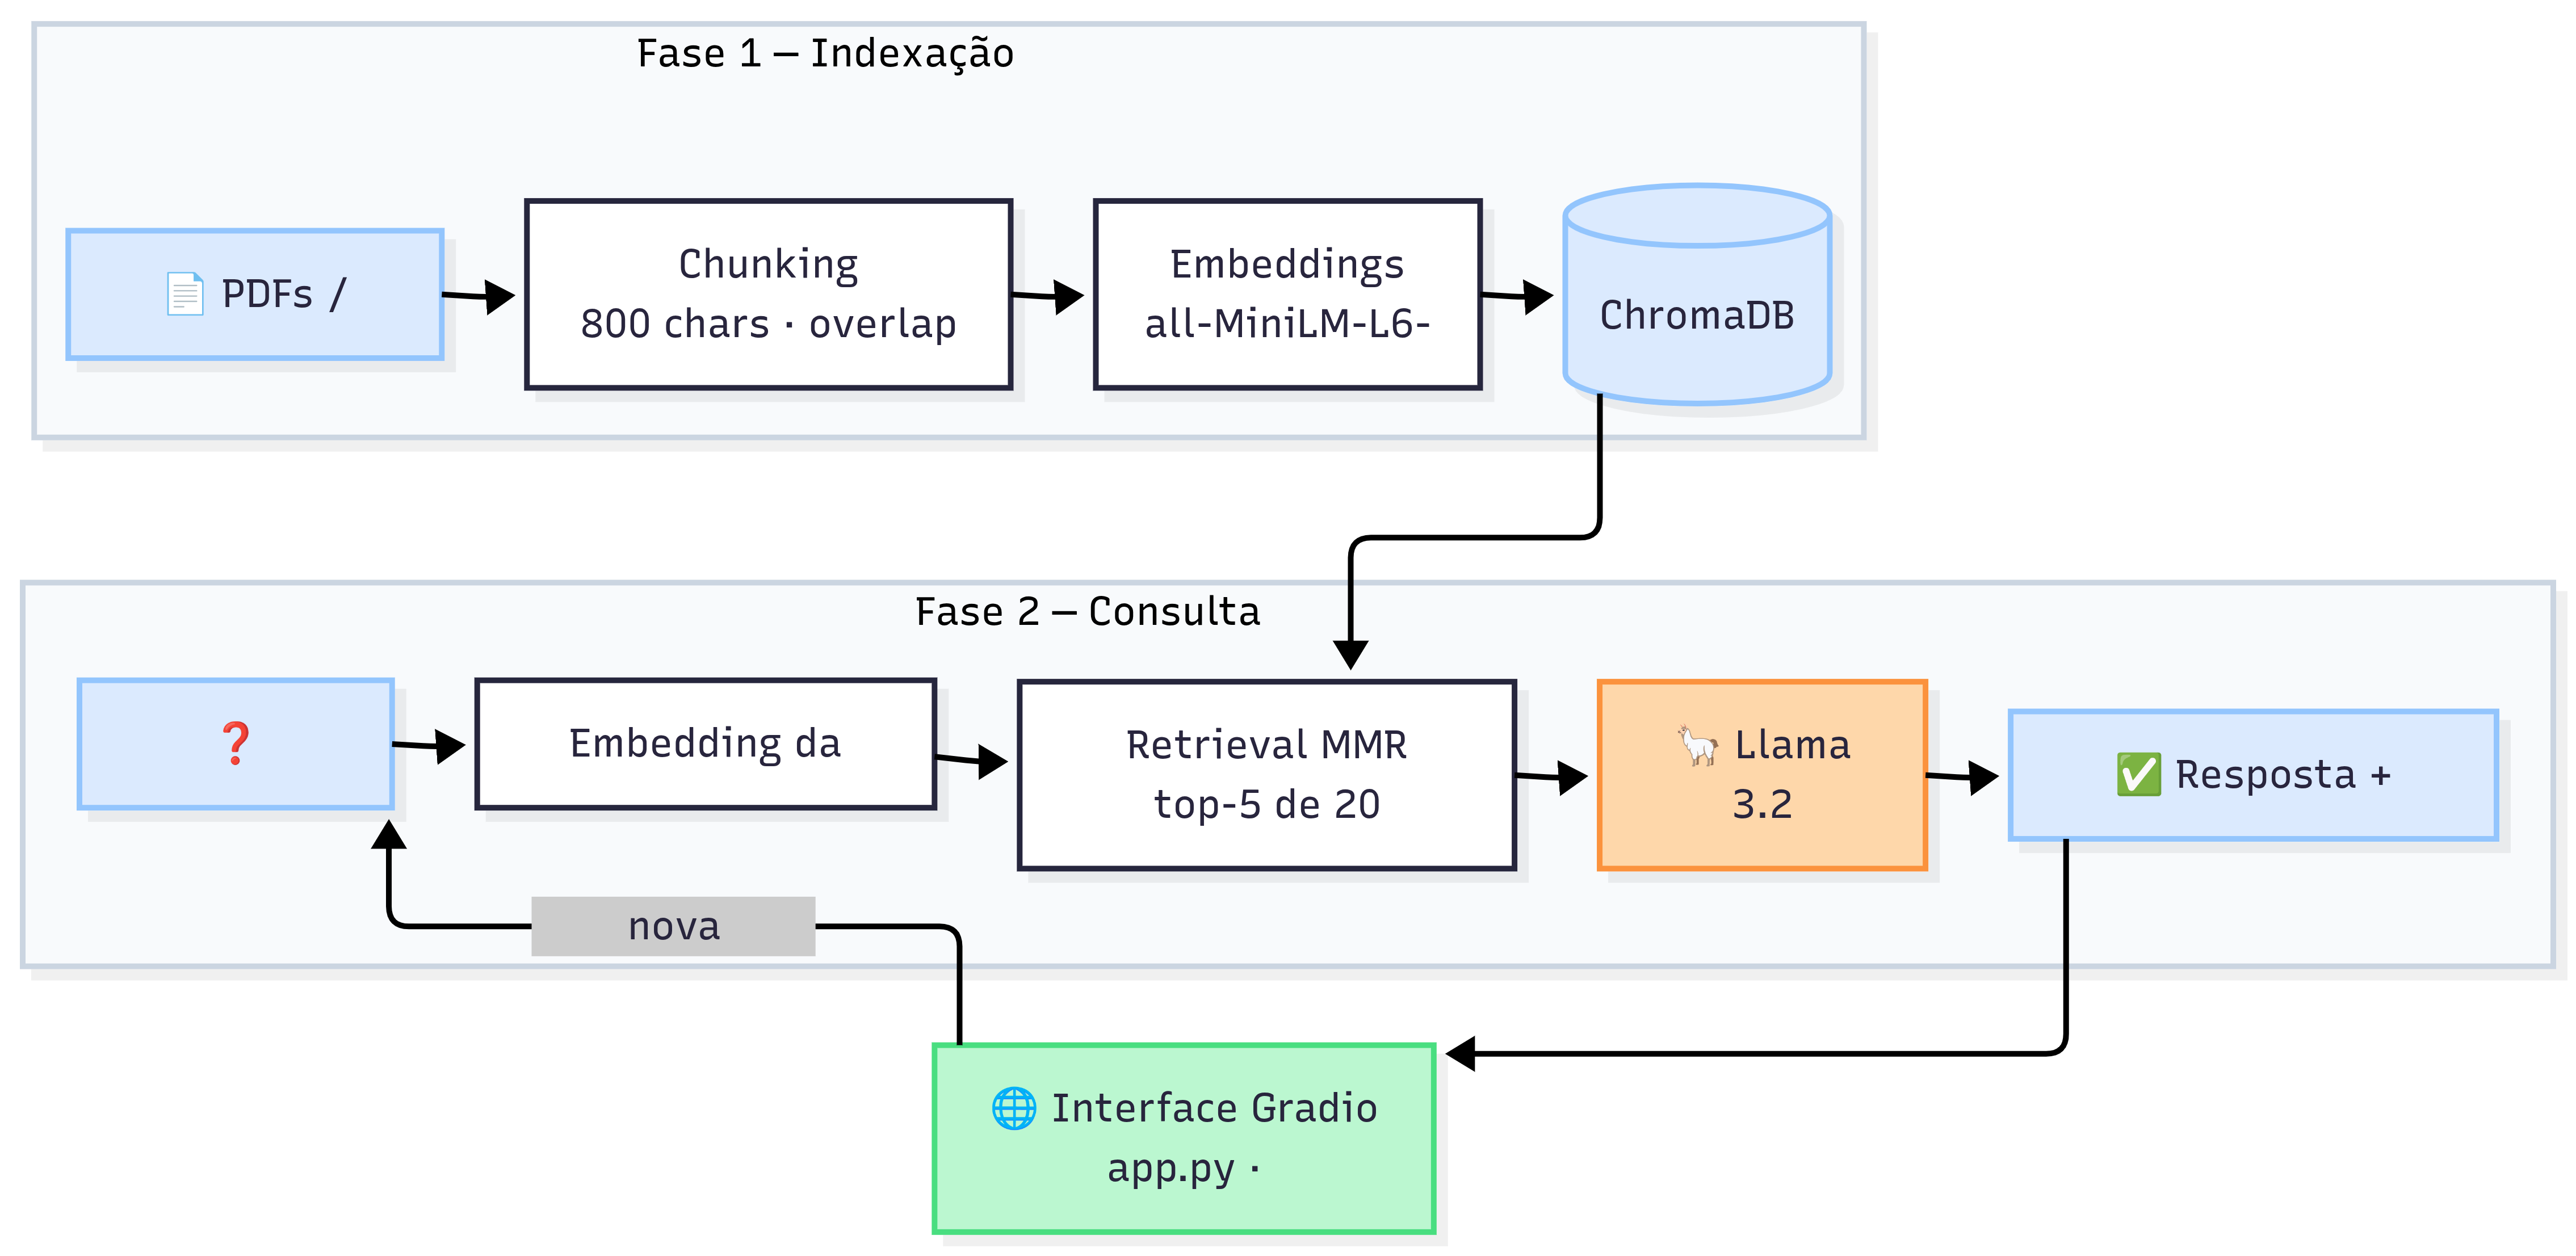
\includegraphics[width=\linewidth]{diagrama.png}
  \caption{Arquitetura do sistema RAG local.}
  \label{fig:arq}
\end{figure}

A separação entre indexação, consulta e interface facilita testes independentes
e evita duplicação de lógica. As funções de embeddings e ChromaDB em
\textbf{\texttt{rag\_base.py}} são guardadas em cache com \texttt{lru\_cache}, evitando
reinicializações desnecessárias entre perguntas.
% ---------------------------------------------------------------------------
\section{Implementação}
% ---------------------------------------------------------------------------

\subsection{Indexação e Chunking}

O \texttt{indexar.py} lê PDFs com \texttt{PyPDFLoader} e ficheiros de texto com
\texttt{TextLoader}. Os documentos são divididos em chunks de 800 caracteres com
overlap de 80, usando \texttt{RecursiveCharacterTextSplitter} com separadores
hierárquicos (\texttt{\textbackslash n\textbackslash n}, \texttt{\textbackslash n},
\texttt{.}, espaço). O overlap preserva contexto nas fronteiras entre chunks, onde
informação relevante poderia ficar artificialmente separada.

Os embeddings são gerados com \texttt{sentence-transformers/all-MiniLM-L6-v2}
\cite{minilm}, com normalização de vetores e batch size de 64. Os vetores são
persistidos em disco no ChromaDB. A orquestração do pipeline é feita com
LangChain \cite{langchain}.

\paragraph{Indexação incremental.} Para evitar reindexação desnecessária, o sistema
mantém um manifesto em \texttt{chroma\_db/index\_manifest.json} com tamanho,
data de modificação e parâmetros relevantes de cada ficheiro. Existem três modos
de operação:

\begin{itemize}
  \item \textbf{skip} --- documentos e parâmetros inalterados; indexação ignorada;
  \item \textbf{incremental} --- apenas os ficheiros novos são processados e
        adicionados ao ChromaDB existente;
  \item \textbf{full} --- ficheiros alterados ou removidos, ou parâmetros
        modificados, desencadeiam reconstrução completa numa pasta temporária,
        que só substitui a base existente após conclusão bem-sucedida.
\end{itemize}
\newpage
\subsection{Recuperação com MMR}

Inicialmente a recuperação usava similaridade vetorial simples. Verificou-se que
em perguntas formuladas de forma diferente dos slides, o sistema devolvia chunks
redundantes do mesmo tópico. Para resolver este problema, adoptou-se Maximal
Marginal Relevance (MMR) \cite{mmr}, configurado em \texttt{rag\_base.py}:

\begin{lstlisting}
RAG_TOP_K=5         # chunks finais enviados ao modelo
RAG_MMR_FETCH_K=20  # candidatos iniciais considerados
RAG_MMR_LAMBDA_MULT=0.5  # equilibrio relevancia/diversidade
\end{lstlisting}

O MMR recolhe 20 candidatos e seleciona os 5 finais maximizando simultaneamente
a similaridade com a query e a diferença entre os chunks já escolhidos. Esta
alteração não exige reindexação, pois atua apenas na fase de pesquisa.

\subsection{Geração de Respostas}

As respostas são geradas com \texttt{llama3.2} via Ollama \cite{ollama},
configurado em \texttt{rag\_base.py} com temperatura 0.1 para favorecer
respostas estáveis. O parâmetro \texttt{RAG\_NUM\_PREDICT=256} limita o
comprimento das respostas, melhorando a latência. O \texttt{keep\_alive=10m}
mantém o modelo carregado em memória entre perguntas, reduzindo a latência das
consultas subsequentes.

Os prompts estão definidos em ficheiros separados por idioma. Ambos instruem o
modelo a responder apenas com base no contexto recuperado e a indicar
explicitamente quando a informação não está disponível nos documentos. Esta
separação, implementada em \texttt{consulta\_pt.py} e \texttt{consulta\_en.py},
torna o comportamento por idioma previsível e fácil de ajustar sem alterar a
lógica central.

\subsection{Interface Web}

\begin{figure}[h]
  \centering
  \includegraphics[width=0.85\textwidth]{2.png}
  \caption{Interface Web.}
  \label{fig:arq}
\end{figure}


A interface foi construída em Gradio \cite{gradio} (\texttt{app.py}) e fica
disponível em \texttt{localhost:7860}. A disposição divide-se em duas áreas:
uma barra lateral para gestão de documentos e um painel principal de chat.

Na barra lateral, o utilizador pode carregar ficheiros PDF ou TXT, escolher o
idioma de resposta (português ou inglês), indexar os documentos carregados e
limpar a base de embeddings sem apagar os documentos originais. A indexação e
a limpeza da base são operações explícitas e independentes, evitando
reindexações acidentais.

No painel de chat, o utilizador escreve uma pergunta e recebe uma resposta
gerada pelo modelo com base nos documentos indexados. Cada resposta inclui
as fontes consultadas, apresentadas num bloco recolhível para não competir
visualmente com o texto principal. A pergunta pode ser enviada com a tecla
Enter ou com o botão \emph{Perguntar}. Existe também um botão para limpar
o histórico da conversa sem afectar a base vetorial.

O pipeline é inicializado automaticamente no arranque da aplicação e
reinicializado após cada reindexação, garantindo que as respostas reflectem
sempre o estado actual dos documentos.

% ---------------------------------------------------------------------------
\section{Configuração e Instalação}
% ---------------------------------------------------------------------------

O projeto pode ser instalado a partir do repositório GitHub:

\begin{lstlisting}
git clone https://github.com/assuncaopaulo7/RAG.git
cd RAG && python3 -m venv venv && source venv/bin/activate
pip install -r requirements.txt
ollama pull llama3.2
python3 indexar.py && python3 app.py
\end{lstlisting}

Os parâmetros podem ser configurados por variáveis de ambiente sem alterar o código:
\texttt{RAG\_DOCS\_DIR}, \texttt{RAG\_CHROMA\_DIR}, \texttt{RAG\_LLM\_MODEL},
\texttt{RAG\_TOP\_K}, \texttt{RAG\_MMR\_FETCH\_K}, \texttt{RAG\_TEMPERATURE},
\texttt{RAG\_NUM\_PREDICT}.

% ---------------------------------------------------------------------------
\section{Testes e Discussão}
% ---------------------------------------------------------------------------

Foram testadas consultas em inglês e português sobre os materiais da unidade
curricular. A pergunta \emph{``What is a RAG?''} devolveu a resposta:
\emph{``A Retrieval-Augmented Generation (RAG) is a technique that helps language
models generate higher-quality outputs by allowing them to look up external,
up-to-date information first.''}, conforme visível na Figura~\ref{fig:chat}.

\begin{figure}[h]
  \centering
  \includegraphics[width=\linewidth]{Screenshot from 2026-06-06 13-53-54.png}
  \caption{Sistema a responder em inglês com indicação das fontes.}
  \label{fig:chat}
\end{figure}

\newpage

Em português, as perguntas produziram respostas fundamentadas nos slides
indexados, com indicação das fontes consultadas, como se pode observar na
Figura~\ref{fig:chat2}.

\begin{figure}[h]
  \centering
  \includegraphics[width=\linewidth]{Screenshot from 2026-06-06 14-05-32.png}
  \caption{Sistema a responder em português com indicação das fontes.}
  \label{fig:chat2}
\end{figure}

Durante o desenvolvimento surgiram dois problemas relevantes. O ChromaDB
rejeitava operações de escrita enquanto a aplicação Gradio mantinha conexões
abertas; a solução foi executar a reindexação num subprocesso e limpar o cache
partilhado com \texttt{SharedSystemClient.clear\_system\_cache()} antes e depois
da operação. Verificou-se também uma incompatibilidade com o componente
\texttt{Chatbot} do Gradio 6, cujo formato de mensagens esperado tinha mudado
entre versões; a interface foi ajustada para o formato aceite pela versão
instalada.

A principal limitação é a dependência da qualidade dos chunks e dos embeddings.
Slides com pouco texto, frases fragmentadas e referências visuais não extraídas
pelo leitor PDF limitam a recuperação. Como trabalho futuro, seria útil testar
embeddings multilingues mais robustos (\texttt{multilingual-e5-base},
\texttt{bge-m3}), adicionar um reranker \textit{cross-encoder} e combinar
pesquisa vetorial com BM25 numa abordagem híbrida.

% ---------------------------------------------------------------------------
\section{Conclusão}
% ---------------------------------------------------------------------------

O projeto resultou num sistema RAG funcional e completamente local, capaz de
responder a perguntas em linguagem natural sobre documentos PDF e TXT sem
depender de APIs externas. A combinação de LangChain, ChromaDB, Sentence
Transformers e Ollama permitiu construir um pipeline modular, onde cada
componente pode ser ajustado de forma independente.

As decisões técnicas mais relevantes foram a indexação incremental com manifesto,
que evita trabalho redundante, e a adopção de MMR em substituição da similaridade
vetorial simples, que melhorou a diversidade do contexto recuperado e a
capacidade de responder a perguntas formuladas de forma indireta.

As limitações identificadas---qualidade dos embeddings em português, extracção
imperfeita de texto em slides com conteúdo visual e ausência de avaliação
quantitativa---apontam caminhos para trabalho futuro: embeddings multilingues
mais robustos, reranking com modelos cross-encoder e recuperação híbrida com
BM25. No geral, o sistema cumpriu os requisitos definidos e constitui uma base
sólida para extensões futuras.

\section*{Declaração de IA Generativa}

Na preparação deste trabalho, o autor recorreu a modelos de linguagem de grande
escala como auxílio na organização de conteúdos, geração de código, na elaboração
de rascunhos iniciais e na revisão linguística do texto. Todo o conteúdo produzido
com recurso a estas ferramentas foi subsequentemente revisto e editado pelo autor,
assegurando o seu rigor técnico e coerência académica. O autor assume plena
responsabilidade pelo conteúdo final do presente trabalho.

% ---------------------------------------------------------------------------
\begin{thebibliography}{9}

\bibitem{lewis2020rag}
P. Lewis et al.,
\textit{Retrieval-Augmented Generation for Knowledge-Intensive NLP Tasks},
Advances in Neural Information Processing Systems (NeurIPS), 2020.
\url{https://arxiv.org/abs/2005.11401}

\bibitem{langchain}
LangChain,
\textit{LangChain Documentation},
2024.
\url{https://python.langchain.com}

\bibitem{chromadb}
Chroma,
\textit{ChromaDB --- The AI-native open-source embedding database},
2024.
\url{https://www.trychroma.com}

\bibitem{minilm}
N. Reimers and I. Gurevych,
\textit{Sentence-BERT: Sentence Embeddings using Siamese BERT-Networks},
EMNLP, 2019.
\url{https://arxiv.org/abs/1908.10084}

\bibitem{ollama}
Ollama,
\textit{Ollama --- Run Large Language Models Locally},
2024.
\url{https://ollama.com}

\bibitem{mmr}
J. Carbonell and J. Goldstein,
\textit{The Use of MMR, Diversity-Based Reranking for Reordering Documents
and Producing Summaries},
ACM SIGIR, 1998.

\bibitem{gradio}
A. Abid et al.,
\textit{Gradio: Hassle-Free Sharing and Testing of ML Models in the Wild},
ICML Workshop, 2019.
\url{https://arxiv.org/abs/1906.02569}

\end{thebibliography}

\end{document}